\documentclass[final]{beamer}
%\usepackage{mathabx}
\usepackage{arev}

\usepackage{amsmath,amsthm,amssymb,latexsym,bbding}
\everymath{\displaystyle}
\usepackage{mathtools}
% \boldmath

\usepackage[utf8]{inputenc}
\usepackage{csquotes}
\usepackage[english]{babel}
\usepackage[T1]{fontenc}

% size=a0 for a0
% here is we use quadratic layout
\usepackage[orientation=portrait,size=custom,height=97,width=97,scale=0.93,debug]{beamerposter}
\mode<presentation>
  {
  \usetheme{IPFposter}
  }


%%%%%%%%%%%%%%%%%%%%%%%%%%%%%%%%%%%%%%%%%%%%%%%%%%%%%%%%%%%%%%%%%%%%%%%%%%%%%%
%% definitions for this poster only



%%%%%%%%%%%%%%%%%%%%%%%%%%%%%%%%%%%%%%%%%%%%%%%%%%%%%%%%%%%%%%%%%%%%%%%%%%%%%%
%% biblatex

\usepackage[backend=biber,citestyle=numeric-comp,bibstyle=BIBStyle,%
            sorting=none,doi=false,hyperref=false]{biblatex}
\bibliography{thebib}
\setbeamertemplate{bibliography item}[text]  % set bibliography item, to show 
                                             % the text of the item (as it 
                                             % comes from biblatex);
                                             % otherwise we get these little 
                                             % images



%%%%%%%%%%%%%%%%%%%%%%%%%%%%%%%%%%%%%%%%%%%%%%%%%%%%%%%%%%%%%%%%%%%%%%%%%%%%%%
%% length and layout stuff

\newlength{\columnheight}
\setlength{\columnheight}{97cm}

\setlength\textwidth{\paperwidth}

\newlength{\marginw}
\setlength{\marginw}{4cm}

\newlength{\tw}
\setlength{\tw}{\textwidth}
\addtolength{\tw}{-2\marginw}


\newlength{\colsep}
\setlength{\colsep}{2cm}

\newlength{\colw}
\setlength{\colw}{0.5\tw}
\addtolength{\colw}{-\colsep}


\setlength{\parindent}{0pt}

\setbeamersize{text margin left=0pt,%
text margin right=0pt,%
%sidebar width left=0pt,%
%sidebar width right=0pt,%
%description width=0pt,%
%description width of=0pt,%
%mini frame size=0pt,%
%mini frame offset=0pt%
}

\newenvironment{myTwoColPoster}{%
  \begin{minipage}[t]{\textwidth}%
    \hspace*{\marginw}%
    \hspace*{9.5bp}%  %% dirty trick!!!!
    %\hfill%
    \begin{minipage}[t]{\tw}}%
  {\end{minipage}%
   \hspace*{\marginw}%
   %\hfill%
   \end{minipage}}

\newenvironment{myCol}%
    {\begin{minipage}[t][\columnheight][t]{\colw}}%
    {\end{minipage}}

\newenvironment{textblock}[1]%
    {\begin{block}{\rule[-0.6ex]{0pt}{2.4ex}\raisebox{-0.25ex}[1.6ex]{#1}}%
     \vspace*{5mm}}%
    {\vspace*{5mm}\end{block}}


%%%------------------------------------------------------------------------%%%
%% the document
%%--------------------------------------------------------------------------%%

%% logos
\logoleft{
\includegraphics[keepaspectratio=true,width=9cm]{fig/logos/dd1_1.pdf}}
\logoright{
\includegraphics[keepaspectratio=true,width=9cm]{fig/logos/dd1_2.pdf}}

%% title
  \title[Fancy Posters]{{\huge Hochverzweigte Polymere und Fraktale}}
  \author[]{\Large Ron Dockhorn\inst{1,2} \and Martin Wengenmayr\inst{1,2}
    \and Jens-Uwe Sommer\inst{1,2}} \institute[IPFdd UBS]{ \inst{1}Leibniz-Institut f\"ur
    Polymerforschung Dresden e. V., Hohe Stra\ss e
    6, 01069 Dresden, Germany\\
    \inst{2}Technische Universit\"at Dresden, Institut f\"ur Theoretische Physik, 01069 Dresden, Germany\\
    ~\vspace{1ex} } \date{}

%% set text in footline
\footlinetext{\texttt{http://www.ipfdd.de}\hfill\texttt{dockhorn@ipfdd.de, wengenmayr@ipfdd.de, sommer@ipfdd.de}}


%%--------------------------------------------------------------------------%%
%% content
\begin{document}
\begin{frame}[t]{}
\begin{myTwoColPoster}
% ---------------------------------------------------------%
% first column
\begin{myCol}
  \begin{textblock}{1. Vielfalt der Polymere: Ketten, Sterne, Fraktale und mehr}
    \begin{minipage}[c]{0.49\textwidth}
      \begin{itemize}\setlength\itemsep{1.4em}\large
        \item einfachstes Polymer: lineare Kette aus einfachen Monomeren
        \item Fraktale Dimension $D_\text{f}$ für Polymermodell \textit{geschwollene Kette}, 
        d. h. Monomere haben ein Eigenvolumen und ein gutes Lösungsmittel umgibt die Kette:
        \begin{align*}
          R &\sim N^{3/5} & D_\text{f}=\frac{5}{3} > 1
        \end{align*}
        \item Einführung von \textbf{\textcolor{IPForange}{Verzweigungen entlang der Kette}} $\Rightarrow$ Veränderung der fraktalen Dimension möglich
      \end{itemize}
    \end{minipage}\hfill
    \begin{minipage}[c]{0.5\textwidth}
      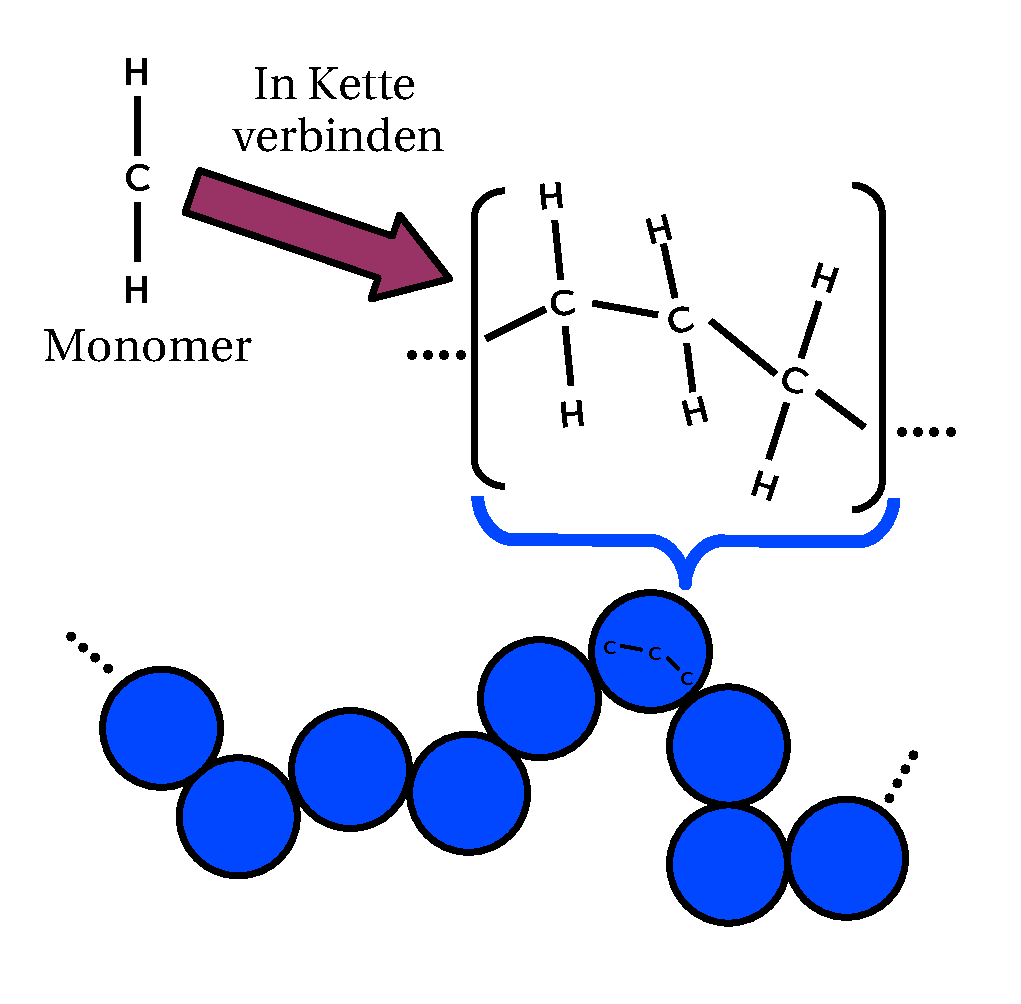
\includegraphics[width=0.8\textwidth]{fig/monchain.pdf}
    \end{minipage}
    \vspace*{1.5cm}
    \begin{center}
      \textbf{\Large Große Vielfalt möglicher Verzweigungen:}
      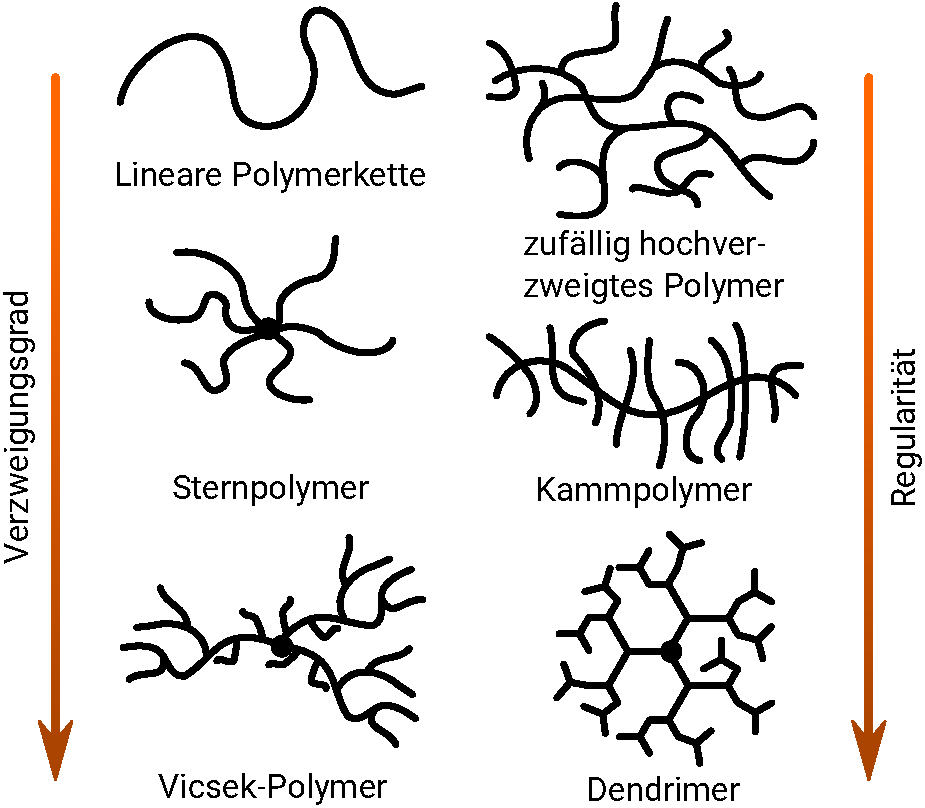
\includegraphics[width=0.8\textwidth]{fig/PolymerTypes_DE2}
    \end{center}
  \end{textblock}

  \begin{textblock}{2. Spezielle Verzweigungsarten: Vicsek Fraktale}
    \begin{itemize}\setlength\itemsep{1.4em}\large
      \item flaches Vicsek Fraktal: ein Quadrat wird von einem 3x3 Gitter überlagert und je vier Teile werden entfernt
    \end{itemize}
      \begin{center}
        
\includegraphics[width=0.9\textwidth]{fig/vicsek_construction}
      \end{center}
    \begin{itemize}\setlength\itemsep{1.4em}\large
      \item Anwendung: bei kompakte Funkantennen, zum Beispiel für Smartphones 
      \item Mit verschiedenen Funktionalitäten in zwei und drei Dimensionen konstruierbar
    \end{itemize}
    \vspace*{3cm}
    $\Rightarrow$ \textbf{\textcolor{IPForange}{\Large Möglichkeit für Synthese von Polymeren mit wohldefinierter Struktur und Dimension}}
  \end{textblock}

\end{myCol}
% ---------------------------------------------------------%
% end the column
% \hspace*{\colsep}%
\hfill
% ---------------------------------------------------------%
% second column
\begin{myCol}
  
  \begin{textblock}{3. Spezielle Hochverzweigte Polymere: Vicsek Polymere\cite{Werner2011}}
    \begin{itemize}\setlength\itemsep{1.4em}\large
      \item Forschung an Synthese von Polymeren nach der Konstruktion eines Viscek Fraktals
      \item Theoretische Untersuchung: 
      \printbibliography
    \end{itemize}
  \end{textblock}

  \begin{minipage}[c]{0.48\textwidth}
    {\centering{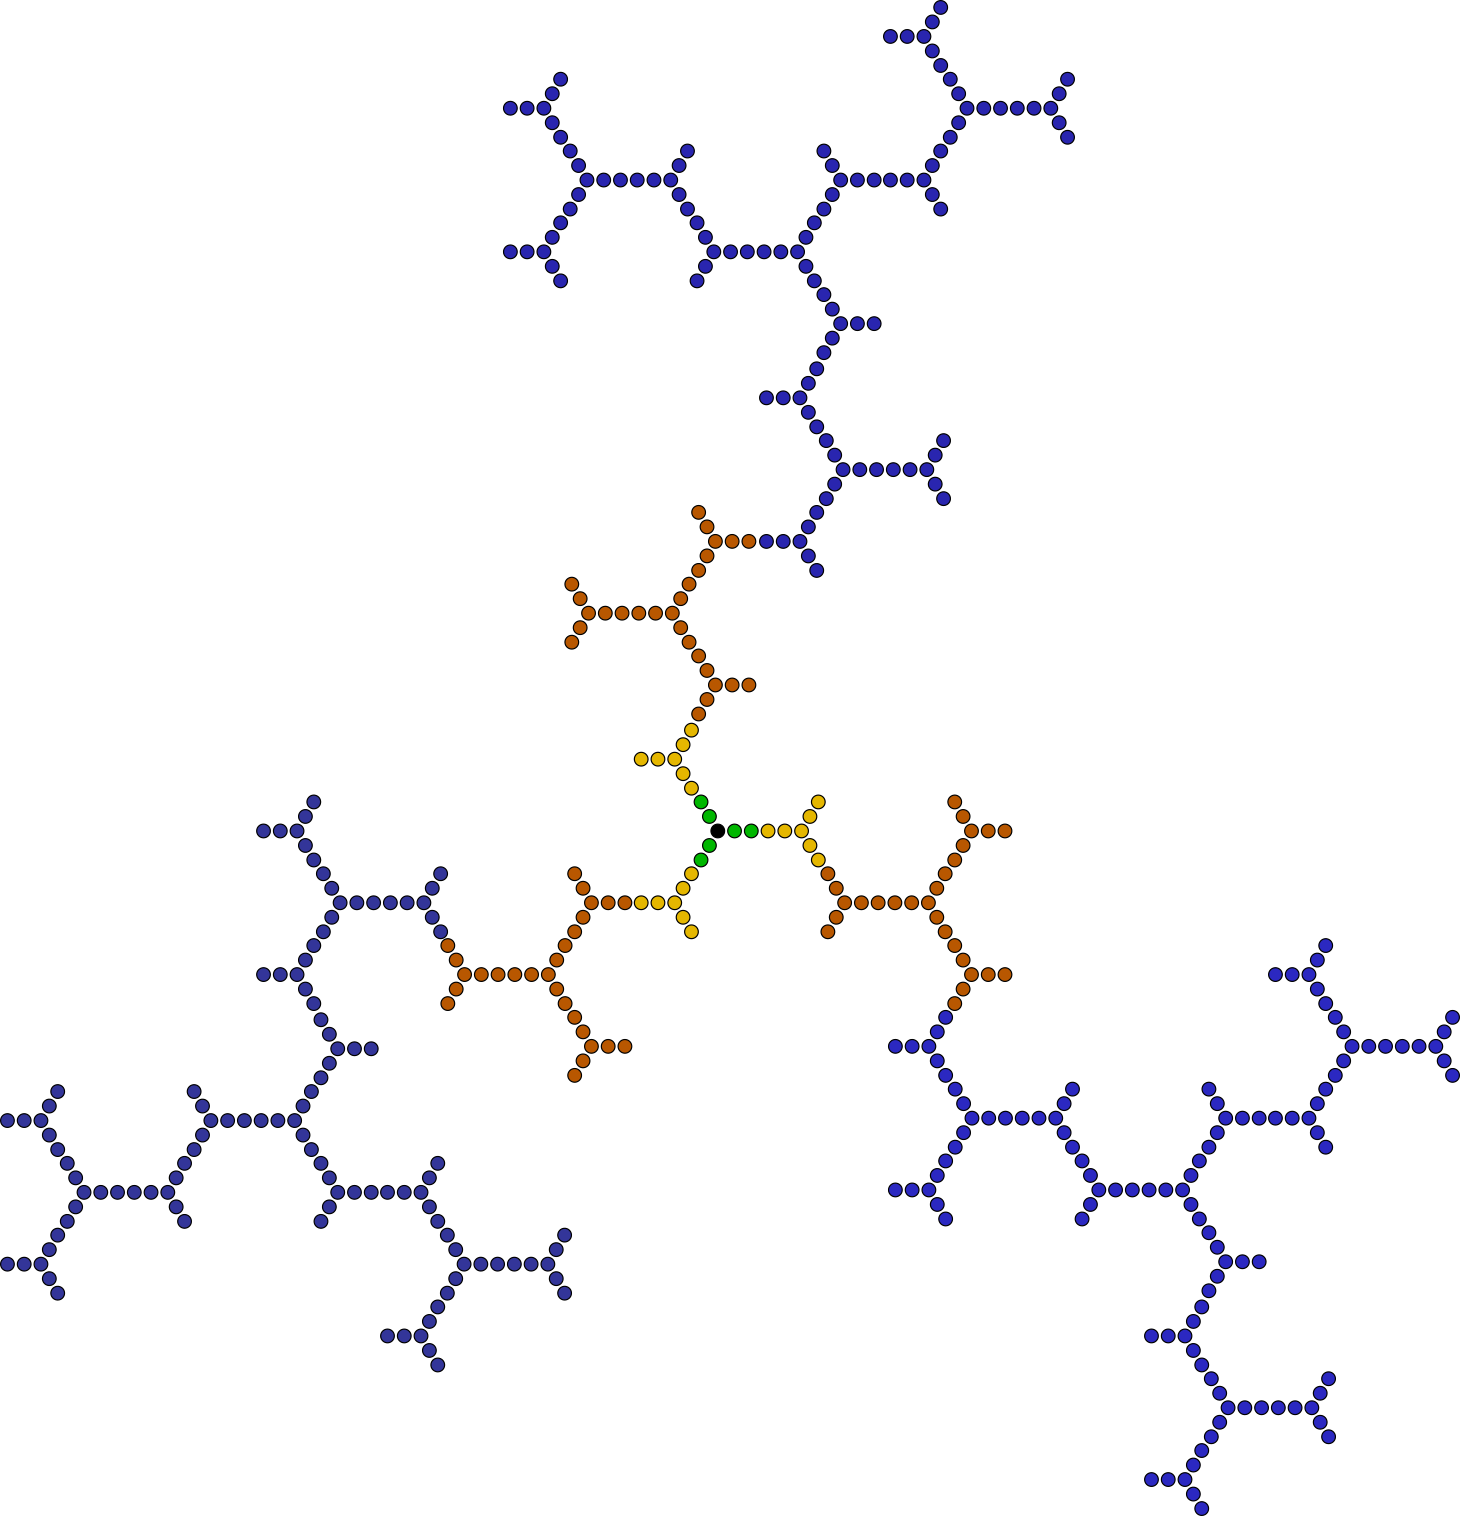
\includegraphics[width=1.1\textwidth]{fig/Vicsek_f3}}}\\
    3-funktionales Vicsek Polymer\\
    Haussdorf Dimension:
    \begin{align*}
      D_\text{f}=\frac{\ln{f+1}}{\ln{3}} = \frac{\ln{4}}{\ln{3}} = 1.16
    \end{align*}
  \end{minipage}
  \hfill
  \begin{minipage}[c]{0.48\textwidth}
    4-funktionales Vicsek Polymer\\
    Haussdorf Dimension:
    \begin{align*}
      D_\text{f}=\frac{\ln{f+1}}{\ln{3}} = \frac{\ln{5}}{\ln{3}} = 1.46
    \end{align*}
    \vspace*{4cm}
    {\centering{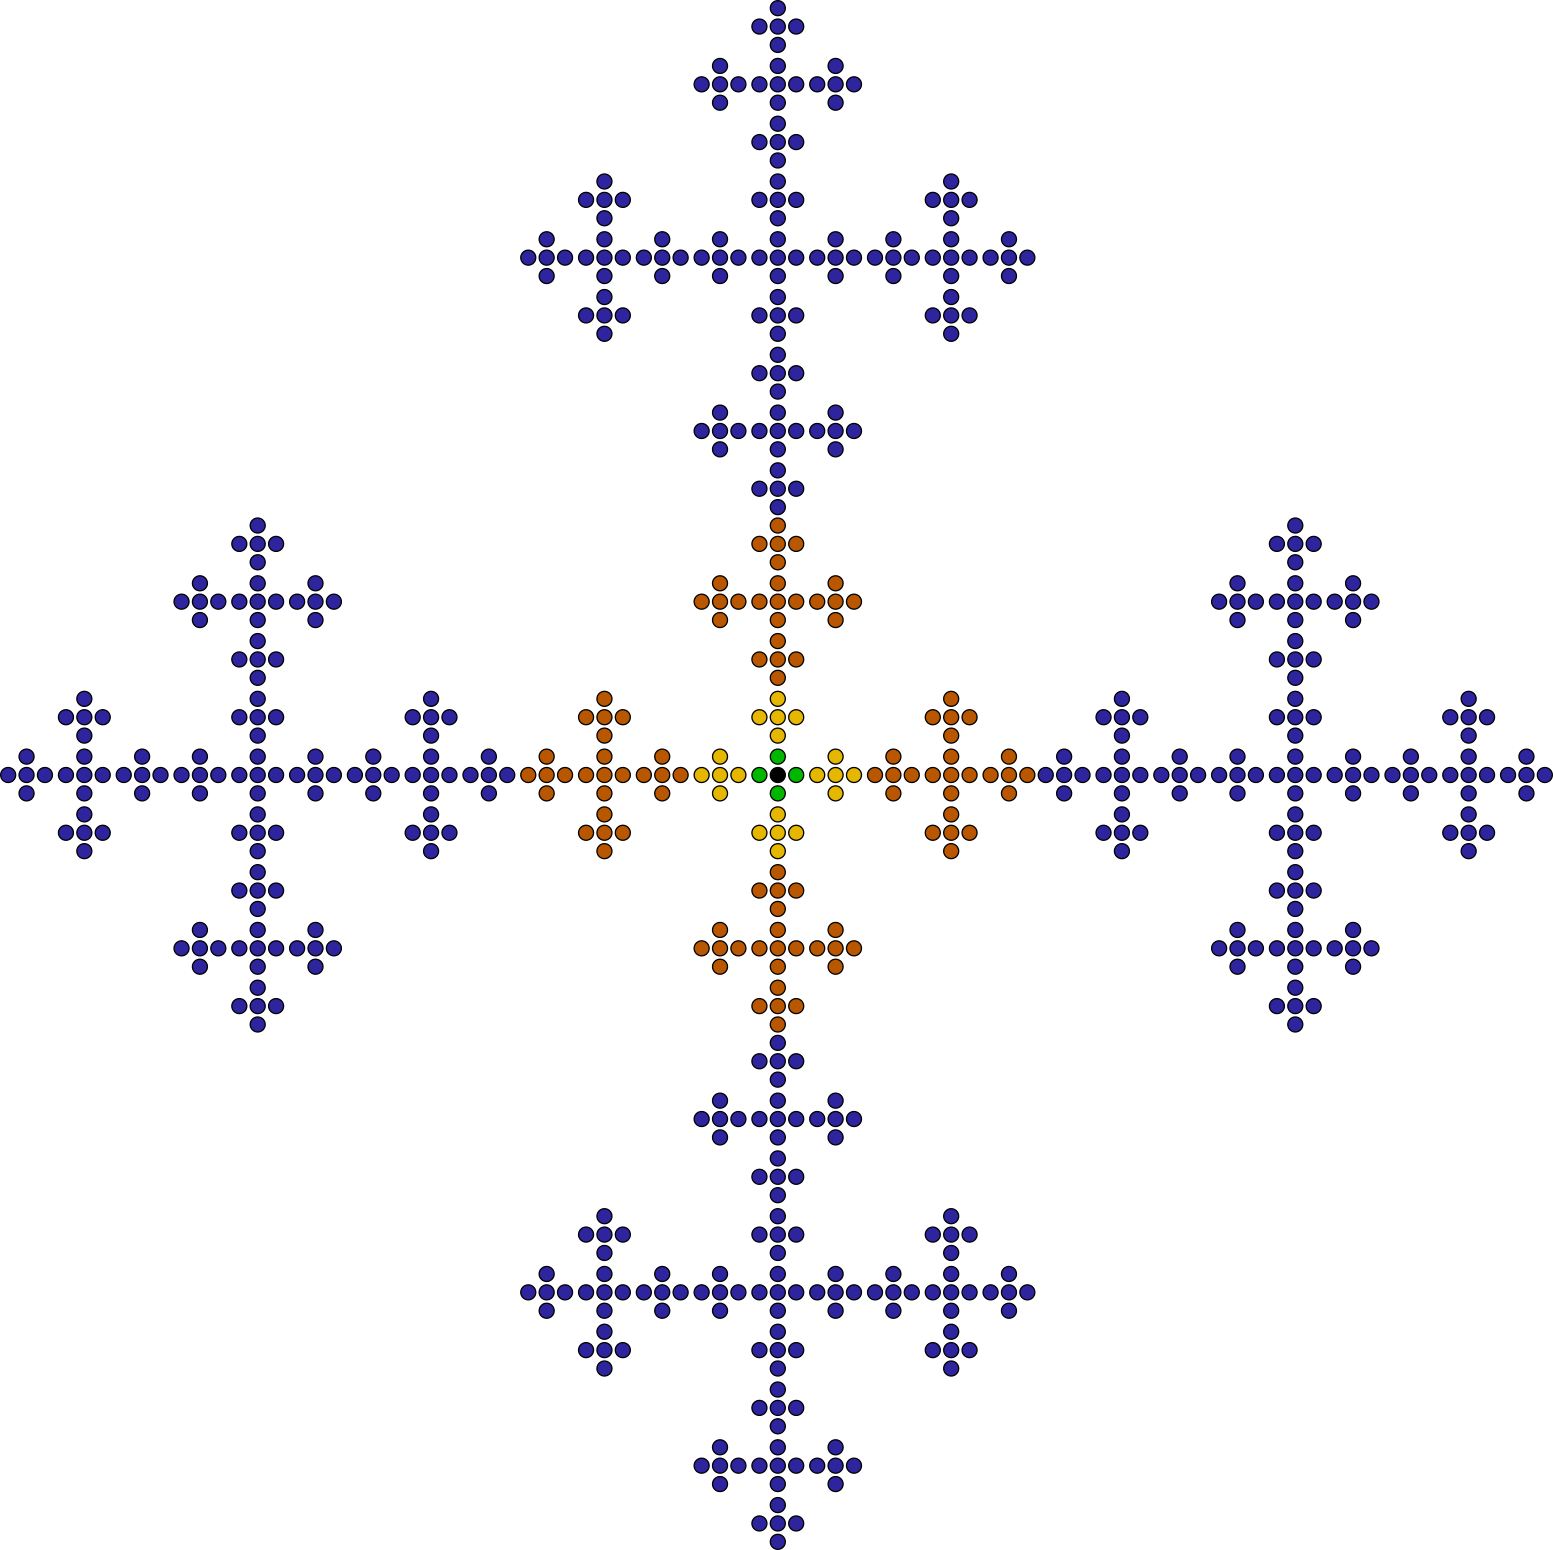
\includegraphics[width=1.1\textwidth]{fig/Vicsek_f4}}}
  \end{minipage}

  \begin{textblock}{4. Jenseits der Fraktalen Dimension: Dendrimere}
    \begin{itemize}\setlength\itemsep{1.4em}\large
      \item Dendrimere sind \textit{baumartig regelmäßig verzeigte} Polymere mit \textbf{regelmäßiger Struktur}, aber \textbf{ohne Selbstähnlichkeit}
      %\item Charakterisiert durch Anzahl der Verzweigungspunkte (die \textit{Generation}), die Anzahl Ketten pro Verzweigungspunkt (die \textit{Funktionalität}) und die Länge der Ketten zwischen den Verzweigungspunkten (die \textit{Spacer})
      \item diese Moleküle sind \textcolor{IPForange}{überraumfüllend}\\
      $\Rightarrow$ mit steigender Generation steigt ihr Platzbedarf stärker, als der zur Verfügung stehende Raum
    \end{itemize}
    \begin{center}
      \textbf{Schematische Darstellung eines Dendrimers} mit dreifunktionalen Verzweigungspunkten\\[2cm]
      
\includegraphics[width=0.55\textwidth]{fig/Dendrimer}
    \end{center}
    \begin{minipage}[c]{0.8\textwidth}
      \begin{center}\large
        \textbf{\textcolor{IPForange}{\Large Die Exponate zeigen zwei Dendrimere:}}
          \begin{itemize}\large
            \item klein mit \textbf{128 Monomeren}, viel freier Raum
            \item groß mit \textbf{2048 Monomeren}, dicht gepackt in der letzten Generation
          \end{itemize}
      \end{center}
    \end{minipage}\hfill
    \begin{minipage}[c]{0.19\textwidth}
      \centering{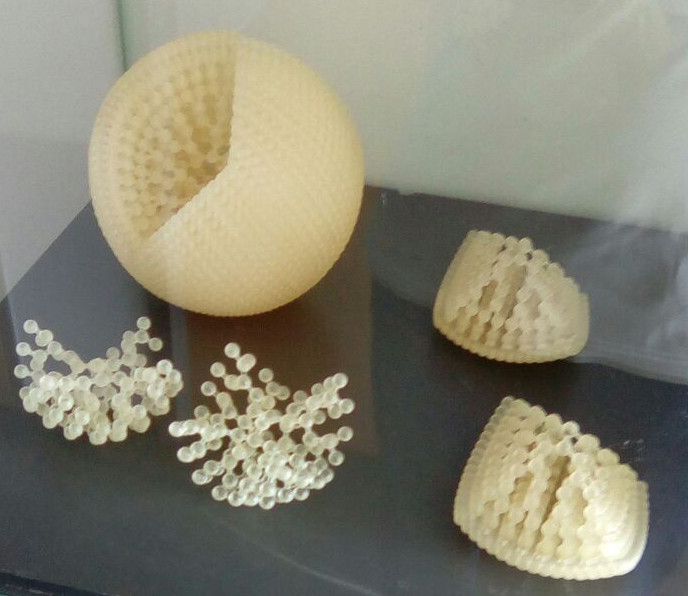
\includegraphics[width=0.8\textwidth]{fig/20180416_exponate_dendrimere}}
    \end{minipage}
  \end{textblock}


\end{myCol}%
\end{myTwoColPoster}
\end{frame}
\end{document}


%%% Local Variables:
%%% compile-command: "rake makepdf"
%%% End:
